\section{Background}

%%In order to calculate the shutdown dose rate of a nuclear systems,
%%a nuclear inventory must be calculated

\subsection{Nuclear Inventory Analysis}
When a material is irradiated a variety of reactions can happen. These 
reactions may lead to production of radionuclides which can persist
after shutdown of the device. For Shutdown Dose Rate (SDR) Analysis, 
the nuclear inventory must be known
in order to quantify the photon emission density as a function of time.

The rate of change in the concentration of nuclide $i$ is given by the 
difference between the production rate and destruction rate of that nuclide.
The rate in which a nuclide undergoes transmutation to some other nuclide
is proportional to its concentration. 
\begin{equation}\label{rate_change_i}
  \frac{dN_{i}(t)}{dt} = \sum_{j} N_{j}(t)P_{j \rightarrow i, total}
  - \sum_{j} N_{i}(t)P_{i \rightarrow j, total}
\end{equation}
Transmutation can occur via a nuclear reaction or a decay. The total
proportionality constant is given by Equation \ref{total_p_const}.
\begin{equation}\label{total_p_const}
  P_{i \rightarrow j, total} = P_{i \rightarrow j, reaction } +
  P_{i \rightarrow j, decay}
\end{equation}
For the reaction process, the proportionality constant is given by
Equation \ref{reaction_p_const}
\begin{equation}\label{reaction_p_const}
  P_{i \rightarrow j, reaction } =
  \int_{E_{n}} \sigma_{i \rightarrow j}(E_{n})
  \phi_{n}(E_n)dE_{n}
\end{equation}
where $\sigma_{i \rightarrow j}(E_{n})$ is the microscopic cross
section for the reaction that transforms nuclide $i$ into $j$, and
 $\phi_{n}(E_{n})$ is the neutron flux for energy $E_{n}$.
For the decay process the proportionality constant is given by Equation
\ref{decay_p_const}

\begin{equation}\label{decay_p_const}
  P_{i \rightarrow j, decay} = \lambda_{i} b_{i \rightarrow j}
\end{equation}
where $\lambda_{i}$ is the decay constant and $b_{i \rightarrow j}$ is
the branching ratio.For entire network of nuclides,
Equation \ref{rate_change_i} can be expressed as
a systems of linear differential equations and is represented by Equation
\ref{rate_change_all}
\begin{equation}\label{rate_change_all}
  \frac{d\vec{N}(t)}{dt} =\boldsymbol{A}  \vec{N}(t)
\end{equation}
where $\vec{N}(t)$ is the vector of all nuclide concentration and $boldsymbol{A}$
is the transfer matrix of production and destruction rates. The solution to this
system of equations is given by Equation \ref{rate_change_sol}.
\begin{equation}\label{rate_change_sol}
  \vec{N}(t) =\vec{N}_{o} e^{\boldsymbol{A}t}
\end{equation}

\subsubsection{Nuclide concetration equations}
This section is primarily to write out equations that might be
important to include when talking about the mesh radionuclide
workflow.
%%
%%
The rate of change of nuclear concentration is given by
\begin{equation}\label{eq:nuclide_conc_rc}
    \frac{dN_{i}(t)}{dt} = \sum_{j} N_{j}(t)P_{j \rightarrow i, total}
    - \sum_{j} N_{i}(t)P_{i \rightarrow j, total}
\end{equation}
%%
%%
For multiple nuclides this becomes a system of differential equations and
can be represented in the following notation
\begin{equation}\label{eq:nuclide_conc_rc_vec}
  \frac{d\vec{N}(t)}{dt} =\boldsymbol{A}  \vec{N}(t)
\end{equation}
%%
%%
A solution to the system of differential equations is given by equation \ref{eq:rate_change_sol}
\begin{equation}\label{eq:rate_change_sol}
  \vec{N}(t) =\vec{N}_{o} e^{\boldsymbol{A}t}
\end{equation}
A way to solve Equation \ref{eq:rate_change_sol} is to break the transmutation network
into a collection of linear chains so that each isotope has one production term and
one destruction term making the $\boldsymbol{A}$ matrix bidiagonal allowing a solution
in the form of the Bateman Equation.
\begin{equation}\label{eq:bateman}
  N_{i}(t) = \sum_{j=1}^{i} N_{j}(0)
  \Bigg[ \Bigg( \prod_{k=j}^{i-1} P_{k} \Bigg)
  \sum_{k=j}^{i}\frac{e^{-d_{k}t}}{\displaystyle \prod_{l=j,\neq k}^{i}(d_{l} -d_{k})}
  \Bigg]
\end{equation}
where $d$ represents the destruction term and $P$ the production   term
%%
%%
When there is not nuclear data available, like is the case for high energy interactions,
another term is introduced in Equation \ref{eq:nuclide_conc_rc}. This term is a
production rate constant.
\begin{equation}\label{eq:nuclide_conc_rc_he}
    \frac{dN_{i}(t)}{dt} = \sum_{j} N_{j}(t)P_{j \rightarrow i, total}
    - \sum_{j} N_{i}(t)P_{i \rightarrow j, total} + Y_{i}
\end{equation}
%%
%%
The system of differential equations can be represented by
Equation \ref{eq:nuclide_conc_rc_vec_he}
\begin{equation}\label{eq:nuclide_conc_rc_vec_he}
  \frac{d\vec{N}(t)}{dt} =\boldsymbol{A}  \vec{N}(t) + \vec{Y}
\end{equation}
%%
%%
A general solution to Equation \ref{eq:nuclide_conc_rc_vec_he} is given below
\begin{equation}\label{eq:rate_change_sol_he}
  \vec{N}(t) =\vec{N}_{o} e^{\boldsymbol{A}t }- \boldsymbol{A^{-1}} \vec{Y}
\end{equation}
If we apply the linear chain method, then the solution is given by Equation
\ref{eq:bateman_he}
\begin{equation}\label{eq:bateman_he}
  \begin{aligned}
  N_{i}(t) = &\sum_{j=1}^{i} N_{j}(0)
  \Bigg[ \Bigg( \prod_{k=j}^{i-1} P_{k} \Bigg)
  \sum_{k=j}^{i}\frac{e^{-d_{k}t}}{\displaystyle \prod_{l=j, \neq k}^{i}
  (d_{l} -d_{k})}
  \Bigg] + &&\\
  &\sum_{j=1}^{i} Y_{j} \Bigg[ \Bigg(\prod_{k=j}^{i-1} P_{k} \Bigg)
  \Bigg(\sum_{k=j}^{i} \frac{1}{\displaystyle \prod_{m=j}^{i} d_{m}} -
  \sum_{k=j}^{i} \frac{e^{-d_{k}t}}{d_{k} \displaystyle \prod_{l=j, \neq k}^{i}(d_{l} -d_{k})}
  \Bigg)\Bigg]
  \end{aligned}
\end{equation}
%%
Another version
\begin{equation}\label{eq:bateman_he_2}
  N_{i}(t) = \sum_{j=1}^{i}
  \Bigg( \prod_{k=j}^{i-1} P_{k} \Bigg)
  \Bigg[ N_{j}(0) \Bigg(\sum_{k=j}^{i}\frac{e^{-d_{k}t}}{\displaystyle
  \prod_{l=j, \neq k}^{i}(d_{l} -d_{k})}
  \Bigg) + Y_{j}
  \Bigg( \frac{1}{\displaystyle \prod_{m=j}^{i} d_{m}} -
  \sum_{k=j}^{i} \frac{e^{-d_{k}t}}{d_{k}
  \displaystyle \prod_{l=j, \neq k}^{i}(d_{l} -d_{k})}
  \Bigg)\Bigg]
\end{equation}
%%
%%
%% CINDER
Cinder solves this equation with a few simplifications. The following identities were used to
simplify the algorithm.
\begin{equation}\label{eq:simplification1}
  \frac{1}{\displaystyle \prod_{m=j}^{i} d_{m}} \equiv
  \sum_{k=j}^{i} \frac{1}{d_{k}
  \displaystyle \prod_{ l=j, \neq k}^{i}(d_{l} -d_{k})}
\end{equation}
%%
\begin{equation}\label{eq:simplification2}
  \sum_{k=j}^{i} \frac{1}{
  \displaystyle \prod_{l=j, \neq k}^{i}(d_{l} -d_{k})} \equiv 0
\end{equation}
%%
%%
Equation \ref{eq:bateman_he2} is reduced to
\begin{equation}\label{eq:bateman_he_simp}
  N_{i}(t) = \sum_{j=1}^{i}
  \Bigg( \prod_{k=j}^{i-1} P_{k} \Bigg)
  \Bigg[ N_{j}(0) \sum_{k=j}^{i}\frac{e^{-d_{k}t}}{\displaystyle
  \prod_{l=j, \neq k}^{i}(d_{l} -d_{k})}
  + Y_{j}
  \sum_{k=j}^{i} \frac{1 - e^{-d_{k}t}}{d_{k}
  \displaystyle \prod_{l=j, \neq k}^{i}(d_{l} -d_{k})}
  \Bigg]
\end{equation}
CINDER90 made it so that there is no need for predefined set
of linear chains. It tests each transmutation step for significance and
constructs the sequences to be calculated. In order to limit the length
of the chains followed, the algorithm only propagates the
initial density and constant production rate to the first nuclide in the sequence.
\begin{equation}\label{eq:bateman_he_1st_n}
  N_{i}(t) =
  \Bigg( \prod_{k=1}^{i-1} P_{k} \Bigg)
  \Bigg[ N_{1}(0) \sum_{k=1}^{i}\frac{e^{-d_{k}t}}{\displaystyle
  \prod_{l=1, \neq k}^{i}(d_{l} -d_{k})}
  + Y_{1}
  \sum_{k=1}^{i} \frac{1 - e^{-d_{k}t}}{d_{k}
  \displaystyle \prod_{l=1, \neq k}^{i}(d_{l} -d_{k})}
  \Bigg]
\end{equation}
%%
%%
which can be written as
\begin{equation}\label{eq:bateman_he_1st_n2}
  N_{i}(t) = \sum_{j=1}^{i}
  \Bigg[ \frac{N_{1}(0) \displaystyle \prod_{k=1}^{i-1} P_{k}}
  {\displaystyle \prod_{k=1, \neq j}^{i}(d_{k} -d_{j})} \Bigg]e^{-d_{j}t} +
  \sum_{j=1}^{i}
  \Bigg [ \frac{Y_{1} \displaystyle \prod_{k=1}^{i-1} P_{k}}
  {\displaystyle \prod_{k=1, \neq j}^{i}(d_{k} -d_{j})} \Bigg]
  \Bigg( \frac{1 - e^{-d_{j}t}}{d_{j}} \Bigg)
\end{equation}


\subsection{Shutdown Dose Rate Analysis}

A primary method to investigate the SDR is known as the
Rigorous 2-Step (R2S) method. The R2S method consists of two transport steps
coupled by an activation step. 
The first transport calculation is performed, and the neutron flux tallied.
The neutron fluxes, and an irradiation scenario are used in an activation
calculation using a dedicated nuclear inventory analysis code to give the 
photon density in the region as function of time. 
This photon density is then used as a source for photon transport,
where the SDR is tallied using a tally modified with flux-to-dose-rate
conversion factors.

\subsection{Shutdown Dose Rate for High Energy Systems}
One of the challenges presented when doing SDR analyses in high energy systems is the 
lack of nuclear cross-section tables in the energies higher than 20 MeV. 
The reaction proportionality constant, Equation \ref{reaction_p_const},
requires the neutron flux and the microscopic cross section of transmuting reaction.
To gap this bridge, some activation codes accept productions and destruction rates
as their input. These production and destruction rates can be obtained from
physics models implemented in MCNP codes.
A radionuclide tally was implemented in MCNP to collect production and destruction
rates in a given geometric cell. The tally is a collision tally and
it collects reaction rates using the physics calculated
cross sections. A reaction rate for any reaction is given by Equation
\ref{reaction_rate_x}

\begin{equation}\label{reaction_rate_x}
  R_{x} = \Sigma_{x} \phi
\end{equation}
where $\Sigma_{x}$ is the  macroscopic cross section for reaction $x$ and
$\phi$ is the scalar flux.
An estimate of the reaction rate is given by Equation \ref{eq:reaction_rate_estimate}
\begin{equation}\label{eq:reaction_rate_estimate}
  R_{x} = \frac{1}{W} \sum_{i \in A} w_{i}
\end{equation}
where $W$ is the total starting weight, $w_{i}$ is the weight before the
collision, $i$ is the index of each event, and $A$ is the set of all events
resulting in reaction $x$.
Equation \ref{eq:reaction_rate_estimate} is easy to implement but can have
high variance and a better tally is needed \cite{OpenMC}.
A collision estimator is a better reaction rate estimator.
An estimate of the flux can be found by using the analog estimator
for a total reaction rate.
\begin{equation}\label{eq:flux}
	\phi = \frac{1}{W} \sum_{i \in C} \frac{w_{i}}{\Sigma_{t}(E_{i})}
\end{equation}
where $C$ is the set of all events resulting in collision with the nucleus,
and  $\Sigma_{t}(E_{i})$ is the total macroscopic cross section of the
target material at the incoming energy of the particle.
From Equation \ref{reaction_rate_x} and Equation \ref{eq:flux}, we can get
a collision estimate of the reaction rate for reaction $x$
\begin{equation}\label{reaction_x_estimate}
  R_{x} = \frac{1}{W} \sum_{i \in A} \frac{w_{i} \Sigma_{x}(E_{i})}{\Sigma_{t}(E_{i})}
\end{equation}
where $\Sigma_{x}(E_{i})$ is the macroscopic cross section for reaction $x$
at the incoming energy of the particle.
The current SDR workflow is seen in Figure \ref{rnucs_r2s}
\begin{figure}[h!]
\begin{centering}
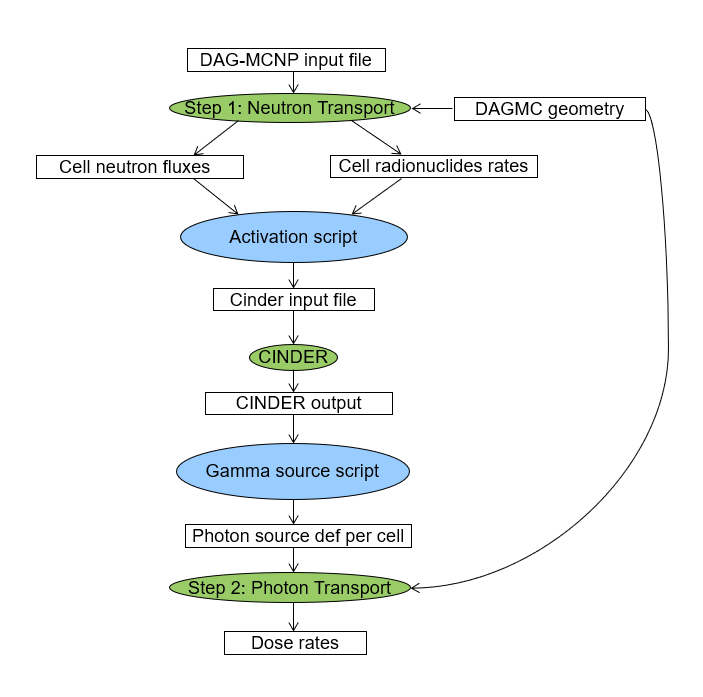
\includegraphics[scale=0.4]{../figs/rnucs_r2s.png}
\caption{Current shut down dose rate workflow for Accelerator systems as used by ORNL}
\label{rnucs_r2s}
\end{centering}
\end{figure}
\newpage
